\begin{exo}{}
	Un satellite situé en un point $S(1\;;\;0)$ observe une planète $P$ qui suit une trajectoire elliptique. \\
	On note $x$ la mesure de l'angle $\widehat{ASP}$.
	\vspace*{2mm}
	\begin{center}
		\begin{tikzpicture}[scale=0.5, x=1cm, y=1cm, >=Triangle]
			\draw[step=1, gray!25, thin] (-7.5,-4.5) grid (7.5,4.5);
			\draw[->, black, thick] (-7.5,0) -- (7.5,0);
			\draw[->, black, thick] (0,-4.5) -- (0,4.5);
			\foreach \x in {-5, 1, 5} { \draw (\x,0.1) -- (\x,-0.1); }
			\node[below] at (-5,-0.1) {\small $-5$};
			\node[below] at (1,-0.1) {\small $1$};
			\node[below] at (5,-0.1) {\small $5$};
			\node[below left] at (0,0) {\small $0$};
			\foreach \y in {1} { \draw (0.1,\y) -- (-0.1,\y) node[left] {\small $\y$}; }
			\foreach \y in {-1} { \draw (0.1,\y) -- (-0.1,\y); }
			\draw[purple, dashed, thick] (0,0) ellipse (6cm and 3cm);
			\fill[purple] (6,0) circle (3pt);
			\node[above right, purple] at (6,0) {A};
			\fill[purple] (0,3) circle (3pt);
			\node[above right, purple] at (0,3) {B};
			\fill[purple] (-6,0) circle (3pt);
			\node[above left, purple] at (-6,0) {C};
			\fill[purple] (0,-3) circle (3pt);
			\node[below right, purple] at (0,-3) {D};
			\coordinate (S) at (1,0);
			\node[above left] at (S) {S};
			\fill[black] (S) circle (3.5pt);
			\coordinate (P) at ({6*cos(35)}, {3*sin(35)});
			\draw[blue!60!gray, thick] (S) -- (P);
			\fill[orange!80!black] (P) circle (4pt);
			\draw[red!60!black, thin] (P) circle (4pt);
			\node[above right, orange!80!black] at (P) {P};
			\begin{scope}[shift={(1,0)}]
				\draw[green!50!black, thick] (1.5,0) arc (0:24:1.5);
				\node[green!50!black, right] at (1.3,0.4) {$x$};
			\end{scope}
			\fill[black] (S) circle (3.5pt);
		\end{tikzpicture}
	\end{center}

	Dans le repère ci-dessus, on a représenté la fonction $d : x \mapsto \text{SP}$ pour $x \in\intff{0}{360}$.
	\begin{center}
		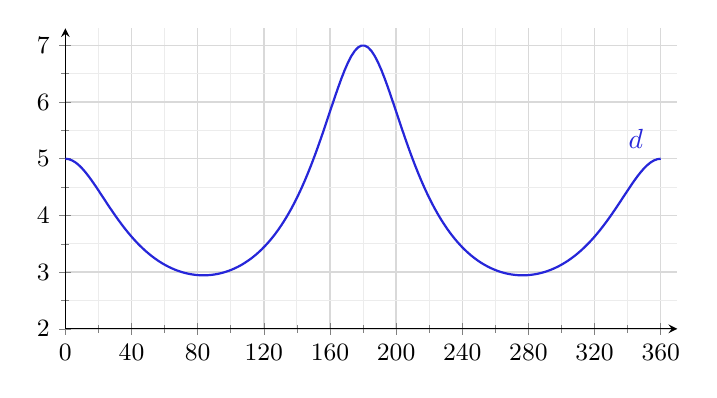
\begin{tikzpicture}
			\begin{axis} [ scale=0.6, x = 0.035cm, y = 1.2cm, xmin = 0, xmax = 370, ymin = 2, ymax = 7.3, axis lines = left, xtick = {0, 40, 80, 120, 160, 200, 240, 280, 320, 360}, ytick = {2, 3, 4, 5, 6, 7}, grid = both, major grid style = {line width=0.5pt, draw=gray!30}, minor tick num = 1, minor grid style = {line width=0.3pt, draw=gray!15}, tick label style = {font=\small} ]
				\addplot[ blue!70!gray, thick, domain=0:360, samples=180, ] { (-cos(x) + sqrt(140 - 104*pow(cos(x),2))) / (4 - 3*pow(cos(x),2)) };
				\node[blue!70!gray, above] at (axis cs:345,5) {$d$};
			\end{axis}
		\end{tikzpicture}
	\end{center}

	\begin{enumerate}
		\item La distance minimale entre $S$ et $P$ se situe-t-elle en $B$ ? Justifier.
		\item Dresser le tableau de variations de $d$ sur l'intervalle $\intff{0}{360}$.
		\item Si la rotation continue, quelle allure aura la courbe de $d$ ?
	\end{enumerate}

\end{exo}
